Problém dvoch obchodných cestujúcich je zjavne NP-úplný, ako to dokázal
už \cite{krarup}, keď tento problém zadefinoval.

V nasledujúcich riadkoch uvedieme niekoľko doterajších výsledkoch, ktoré sa vyskytli
pri riešení tohoto problému.

\section{Aproximačné algoritmy}

Dá sa pomerne ľahko ukázať, že pre problém dvoch obchodných cestujúcich vo všeobecných grafoch
neexistuje aproximačný algoritmus s konštantným aproximačným pomerom. Dôkaz je v prakticky
rovnaký ako pre problém obchodného cestujúceho.

V prípade, že graf spĺňa trojuholníkovu nerovnosť sa už dajú nájsť approximačné algoritmy.
Dá sa napríklad ukázať, že ak má graf dostatočne veľa vrcholov, tak ku každej TSP ceste
existuje TSP cesta, ktorá je s ňou disjuktná a má dĺžku najviac rovnú $(2+\epsilon)$-násobku
dĺžky pôvodnej cesty.
Použítím $1.5$-aproximácie pre problém obchodného cestujúceho (\cite{christofides}) vieme
dostať $(9/4 + \epsilon)$-aproximačný algoritmus. 

Dá dosiahnúť aj $2$-aproximačný algoritmus, ako to je ukázané v \cite{apx2}. Hlavnou
ideou je zostrojiť najprv dve disjuktné kostry s minimálnou cenou pomocou algoritmu
uvedeného v \cite{spanning2} a následne pomerne technickou konštrukciou zostrojiť
s použitím týchto kostier dve disjunktné hamiltonovské kružnice.

V prípade, že ceny hrán môžu byť len z množiny $\{1,2\}$ existuje $11/9$-aproximačný
algoritmus (\cite{gimadi}). V tomto článku sa nachádza navyše niekoľko výsledkov pre 
variáciu problému, kde cenu ciest maximalizujeme.

\section{Riešenia pomocou celočíselného lineárneho programovania}

\subsection{Riešenie problému obchodného cestujúceho pomocou celočíselného
lineárneho programovania}

Najprv zhrnieme niekoľko výsledkov o riešení problému obchodného cestujúceho pomocou
celočíselného lineárneho programovania, ktoré sa nachádzajú v \cite{tspsurvey}.

Problém obchodného cestujúceho sa dá priamočiaro popísať nasledujúcim celočíselným lineárnym
programom:

$$\min \sum_{e \in E} c(e) x_e$$ 

Za predpokladov:
\begin{subequations}
\begin{equation}\forall e \in E: x_e \in \{0, 1\} \label{eq:enum}\end{equation}
\begin{equation}\forall v \in V: \sum_{e \in \delta(v)} x_e = 2 \label{eq:vertexsum1} \end{equation}
\begin{equation}\forall S \subset V, S \neq \emptyset: \sum_{e \in \delta(S)} x_e \geq 2 \label{eq:subtour1}\end{equation}
\end{subequations}

Kde $\delta(v)$ je množina všetkých hrán, ktoré majú koniec vo vrchole $v$ a
$\delta(S)$ je množina všetkých hrán, ktorá majú jeden koniec v $S$ a druhý v $V \setminus S$.

Podmienky \eqref{eq:vertexsum1} zabezpečujú, aby z každého vrchola výchádzali práve
dve hrany. Podmienky \eqref{eq:subtour1} zabezpečujú, aby sme mali iba jeden cyklus.
Táto formulácia má ale exponenciálne veľa podmienok a na prvý pohľad je neužitočná.

Existuje formulácia, ktorá má iba polynomiálne veľa podmienok. V tomto prípade
ale použijeme orientované hrany:

$$\min \sum_{i\neq j} c(i,j) x_{ij}$$

Za predpokladov:
\begin{subequations}
\begin{equation}\forall j \neq i_0: \sum_{i=1}^n x_{ij} = 1\end{equation}
\begin{equation}\forall i \neq i_0: \sum_{j=1}^n x_{ij} = 1\end{equation}
\begin{equation}\forall i,j, i \neq i_0 \vee j \neq j_0: u_i + u_j + nx_{ij} \leq n-1\end{equation}
\end{subequations}

Cieľom premenných $u_i$ je zaviesť očíslovanie vrcholov na kružnici. Tento program
má síce len polynomiálne veľa podmienok, ale ukazuje sa, že nie je ľahko riešiteľné
pomocou bežných nástrojov na riešenie celočíselných lineárnych programov.

Ukazuje sa, že pomerne účinný algoritmus je nasledovný:

\begin{enumerate}
\item Vytvor lineárny program, ktorá obsahuje iba podmienky \eqref{eq:enum}, 
\eqref{eq:vertexsum1}.
\item Najdi riešenie daného lineárneho programu.
\item Ak je riešenie lineárneho programu iba jedna kružnica, tak máme dobré riešenie a skonči.
\item Ináč nájdi porušené podmienky \eqref{eq:subtour1} a pridaj ich do lineárneho
programu. A pokračuj krokom 2.
\end{enumerate}

Tomuto postupu sa zvykne hovoriť aj "subtour elimination".

\subsection{Riešenie problému dvoch obchodných cestujúcich pomocou celočíselného
lineárneho programovania}

V nasledujúcej časti zhrnieme výsledky z \cite{duchenne}.
Priamym rozšírením postupu pre obchodného cestujúceho na dvoch cestujúcich
dostaneme nasledovný program:

$$\min \sum_{e \in E} c(e) x_e + \sum_{e \in E} c(e) y_e$$ 

Za predpokladov:
\begin{subequations}
\begin{equation}\forall e \in E: x_e \in \{0, 1\}\end{equation}
\begin{equation}\forall e \in E: y_e \in \{0, 1\}\end{equation}
\begin{equation}\forall e \in E: x_e + y_e \leq 1\end{equation}
\begin{equation}\forall v \in V: \sum_{e \in \delta(v)} x_e = 2\end{equation}
\begin{equation}\forall v \in V: \sum_{e \in \delta(v)} y_e = 2\end{equation}
\begin{equation}\forall S \subset V, S \neq \emptyset: \sum_{e \in \delta(S)} x_e \geq 2
\label{eq:subtour2}\end{equation}
\begin{equation}\forall S \subset V, S \neq \emptyset: \sum_{e \in \delta(S)} y_e \geq 2
\label{eq:subtour3}\end{equation}
\end{subequations}

Spôsob riešenie je podobný ako pri riešení problému obchodného cestujúceho -- najprv
nepoužijeme žiadne z podmienok \eqref{eq:subtour2}, \eqref{eq:subtour3} a postupne
pridáme len porušené podmienky. V \cite{duchenne} sa tento algoritmus nazýva "3-index".

Ukazuje sa, že tento algoritmus je pomerne pomalý a potrebuje veľa iterácií riešenia
lineárneho programu. Pri praktickom testovaní na náhodných euklidovských grafoch
je tento algoritmus úspešný maximálne pre grafy s $50$ vrcholmi. Hlavným problémom
tohoto algoritmu je, že pomerne často nastáva taký prípad, keď len prehadzujeme hrany z $x$ 
do $y$ a naopak. 

\smallskip

V \cite{duchenne} tento postup ešte vylepšili. Použili algoritmus s nasledujúcou myšlienkou:
Namiesto hľadania dvoch
disjuktných hamiltonovských kružníc budeme hľadať najlacnejší 4-regulárny 4-súvislý podgraf.
Následne ak sa tento podgraf dá rozložiť na dve hamiltonovské kružnice, tak máme riešenie.
Toto sa nemusí vždy podariť, na \ref{fig:bad} je príklad grafu, ktorý je 4-súvislý a 4-regulárny,
ale nemá hamiltonovskú kružnicu. 

\begin{figure}[h]
\centering
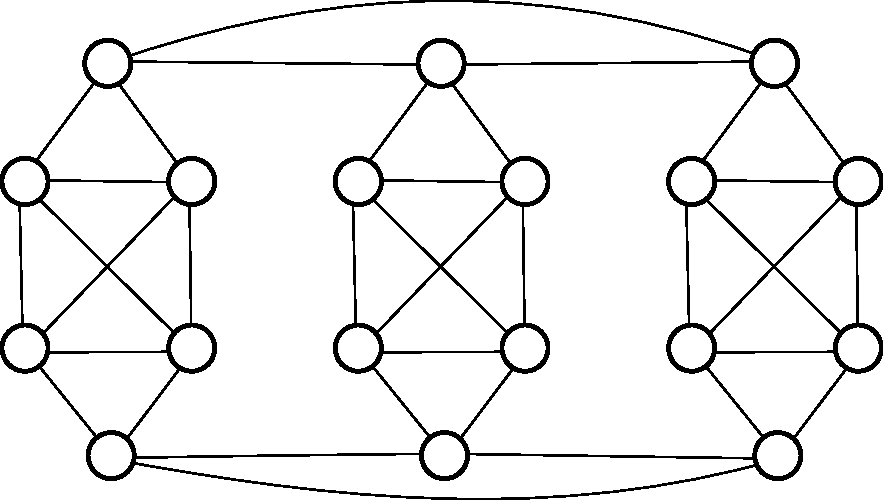
\includegraphics[scale=0.5]{img/bad4.pdf}
\caption{Príklad grafu, ktorý je 4-súvislý a 4-regulárny, ale nie je hamiltonovský.}
\label{fig:bad}
\end{figure}

Ak sa nám nepodarí 4-faktor rozložiť na dve hamiltonovské kružnice, tak tento 4-faktor zakážeme
a budeme hľadať najlacnejší nezakázaný podgraf.
Iný pohľad na tento algoritmus je taký, že v lineárnom programe zlúčíne premenné $x_e$ a $y_e$ 
do jednej, čiže aktuálny program, ktorý budeme nazývať 2-index vyzerá takto:

$$\min \sum_{e \in E} c(e) x_e$$ 

Za predpokladov:
\begin{subequations}
\begin{equation}\forall e \in E: x_e \in \{0, 1, 2\}\end{equation}
\begin{equation}\forall v \in V: \sum_{e \in \delta(v)} x_e = 4\end{equation}
\begin{equation}\forall S \subset V, S \neq \emptyset: \sum_{e \in \delta(S)} x_e \geq 4
\label{eq:subtour4}
\end{equation}
\end{subequations}

Aktuálne už hľadanie porušených podmienok \eqref{eq:subtour4} nie je také jednoduché.
Nestačí už len hľadať komponenty vzniknutého grafu potrebujeme hľadať rezy, ktoré
majú veľkosť menšiu ako 4. Na toto môžeme napríklad použiť algoritmus z \cite{stoer}. 

Väčším problémom je zistenie, či sa dá 4-regulárný 4-súvislý podgraf rozdeliť na dve
disjuktné hamiltonovské kružnice. Tento problém je NP-úplný ako ukázal \cite{hamdecomp}.
V \cite{duchenne} na riešenie tohoto problému používajú upravený 3-index algoritmus.
Takýto 2-index algoritmus funguje pre náhodné euklidovské grafy, ktoré majú menej ako $200$
vrcholov.
